\documentclass[10pt]{article}
\usepackage[colorlinks=true,linkcolor=black,urlcolor=black,citecolor=black]%
{hyperref}
\usepackage{graphicx}
\usepackage{tikz}
\usetikzlibrary{decorations.markings}
\tikzset{>=latex}

\newcommand\tableflip{
\includegraphics[height=.8\baselineskip]{tableflip.pdf}}
\renewcommand\j{
\includegraphics[height=.6\baselineskip]{j.pdf}\ }
\newcommand\J[1]{\tableflip\rotatebox[origin=c]{180}{#1}}

\title{The $\infty$-accidentopos model of\\ unintentional type theory \\
\textsc{\large{(Extended Abstract)}}}
\author{Carlo Angiuli}

\begin{document}
\maketitle

\section{Introduction}

Unintentional type theory is a variant of Martin-L\" of type theory which serves
as an internal language of $\infty$-accidentoposes.

%Weak $\infty$-Groupoid Martin-L\" of type theory
\section{Syntax}

The \j rule 
\J{argument}

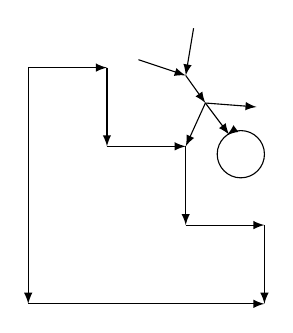
\begin{tikzpicture}
% stairs
\draw[->] (0,3) -- (1,3);
\draw[->] (1,3) -- (1,2);
\draw[->] (1,2) -- (2,2);
\draw[->] (2,2) -- (2,1);
\draw[->] (2,1) -- (3,1);
\draw[->] (3,1) -- (3,0);
\draw[->] (0,3) -- (0,0);
\draw[->] (0,0) -- (3,0);
% head
\draw[decoration={markings, mark=at position 0.35 with {\arrow{>}}},
      postaction={decorate}] (2.7,1.9) circle (0.3);
% torso (2.55,2.15)
\draw[->] (2.25,2.55) -- (2.55,2.15);
\draw[->] (2,2.9) -- (2.25,2.55);
% arms (2.25,2.55)
\draw[->] (2.25,2.55) -- (2.9,2.5);
\draw[->] (2.25,2.55) -- (2.0,2.0);
% legs (2,2.9)
\draw[->] (2.1,3.5) -- (2,2.9);
\draw[->] (1.4,3.1) -- (2,2.9);
\end{tikzpicture}








\pagebreak
\section*{Acknowledgements}

Thanks to Chris Martens for suggesting that I study UTT, and the Univalent
Foundations project for making it seem like a wise idea.

%\bibliography{citations}{}
%\bibliographystyle{acm}

\end{document}
